\end{multicols}

\begin{figure*}[!ht]
    \centering
    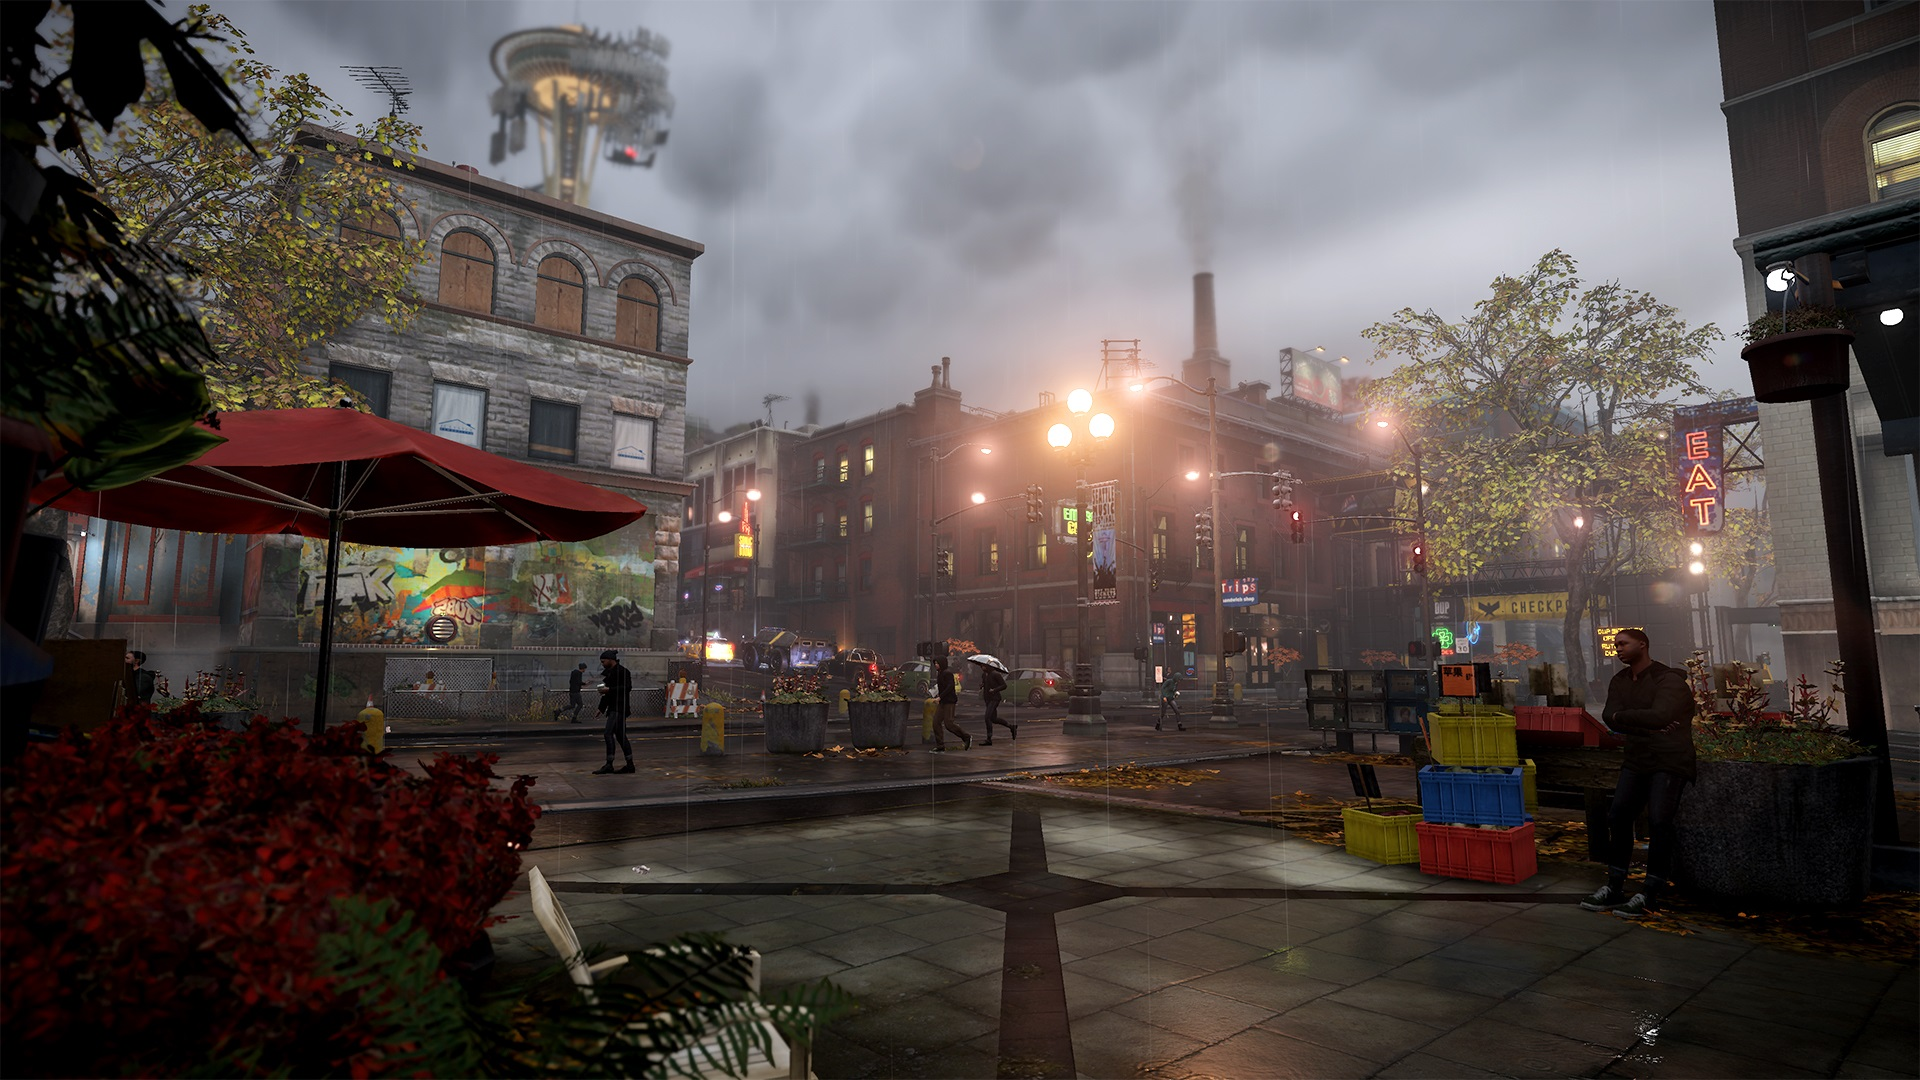
\includegraphics[width=\linewidth]{imagens/cidade_1.jpg}
\end{figure*}

\subsection{\bf História}
Os seres humanos sobreviveram ao Apocalipse por puro "milagre", diversas cidades foram destruídas, florestas queimadas, durante a guerra as armas que foram utilizadas foram suficientes para transformar montanhas em pó, rios e lagos escureceram de cinza e sangue, a radiação que se espalhou pela terra, ar e o que sobrou de água acabou por exterminar boa parte da vida na terra.

O milagre que salvou os humanos chama-se Dominus Corporation, uma empresa que estava estudando um novo material resistente de aparência semelhante a um acrílico para construir bolhas de proteção contra a poluição que o mundo estava sofrendo, pouco antes da guerra essa empresa cresceu consideravelmente e devido a esse crescimento, pode adquirir orçamento suficiente para concluir suas pesquisas e desenvolver a Nephila, com ela foi possível construir algumas cidades Colmeia, como são chamadas, são cidades envoltas num domo de proteção, onde a poluição de fora não consegue penetrar. Nas colmeias a vida continua aparentemente normal, como se o apocalipse nunca tivesse acontecido, as pessoas trabalham, estudam e seguem suas rotinas, a única obrigação é que eles devem tomar algumas pílulas de proteção contra a radiação e passar por exames anuais, pois nada nunca mais vai estar 100\% seguro.

A guerra acabou e o véu foi rasgado, hoje em dia existem mais pessoas dispostas a caçar o sobrenatural do que nos tempos antigos, se um Garou for visto perambulando pelas ruas, ele vai ser tratado como um monstro que merece ser executado, sua cabeça é tão premiada que em uma noite facilmente se juntaria 100 civis e uns 20 caçadores fortemente armados para abater a criatura, só para que assim possam ganhar um pouco de dinheiro vendendo seus restos.

\newpage
\begin{multicols}{2}

\subsection{\bf Cenário}
\imgColuna{imagens/cidade_2.jpg}
\subparagraph*{Colmeias são cidades protegidas com a tecnologia da Dominus Corporation, de formato circular, nelas foram construídos diversos arranha-céus, os mais bem equipados e melhores no geral ficam próximos ao centro, enquanto as “favelas em pé” ficam localizados as margens da colmeia, estas construções foram feitas com o que sobrou dos recursos do mundo e o que sobrou de melhor ficou para os ricos e poderosos. Uma curiosidade sobre os arranha-céus é que sempre o maior deles é chamado de Palácio, sempre localizado no centro da cidade e é comandado por uma Rainha. O clima dentro das colmeias é sempre quente, coisa de 35º com uma variação pequena para mais ou para menos. De dentro da Colmeia não é possível enxergar o mundo exterior.}

\imgColunaLegenda{imagens/cidade.jpg}{Cidade e seus Setores}
\subparagraph*{As cidades são sempre bem protegidas, existem patrulhas de policiais continuamente, a fim de evitar quaisquer conflitos que surjam dentro da Colmeia, afinal de contas, as pessoas precisam sempre obedecer às regras impostas pelas Rainhas.
As colmeias se ligam por meio de túneis subterrâneos, totalmente desconhecidos pela população comum, somente os responsáveis pela preservação destes túneis detêm conhecimento sobre os mesmos. Estes túneis são protegidos por soldados fortemente armados e as vezes por algumas criaturas desconhecidas.}
 
\subsection{\bf Habitantes do Setor 0}
\imgColuna{imagens/civis.jpg}
\subparagraph*{No setor 0 existem o que chamam de "Favelas" são prédios gigantescos com seus 100 andares e seus $4km^2$. Neste setor existe todos os tipos de miseraveis, pessoas simples em que seus antepassados não possuiam influência suficiente para garantir uma boa morádia nesse novo mundo.}
\preencher

\subsection{\bf Penumbra}
\imgColuna{imagens/penumbra.jpg}
\subparagraph*{A visibilidade na penumbra é sempre precária, existe somente a luminosidade de uma pequena luz que é emitida ao alto do domo, que dá um tom avermelhado ao ambiente. Ela também possui climas extremos, durante o dia a o ar é muito denso e quente, a temperatura chega facilmente aos 40º, a dor e o sofrimento é palpável no odor repugnante que exala de cada rua e buraco que possa ser encontrado, é possível sentir o sofrimento de forma intrínseca. A partir das 16 horas o clima muda abruptamente, a temperatura que antes estava em torno dos 40º facilmente vai abaixo dos -10º, os espiritos que se debatiam agora são congelados e ficam totalmente imóveis para que as aranhas possam vir se alimentar deles, elas adquiriram o habito e a habilidade de sugar a essência destes sem que morram, fechando a ferida com uma substância amarela que escretam de suas quelíceras.}

\subsubsection{\bf Espiritos}
\imgColuna{imagens/espirito_torturado.jpg}
\subparagraph*{Ao caminhar pela penumbra das colméias é possível ver espíritos moribundos presos a teias enegrecidas ou avermelhadas, alguns destes com olhares apáticos e vázios que seguem os viajntes livres, enquanto há outros ensandecidos, que se debatem de forma lenta, como se já estivessem cansados de lutar, mas que ainda não desistiram, mas é perceptível que a maioria perdeu sua essência.}

\newpage